\documentclass[a4paper, notitlepage, 9pt]{extreport}
\usepackage[italian]{babel}
\usepackage[T1]{fontenc}
\usepackage[utf8]{inputenc}
\usepackage{amsmath}
\usepackage{amsfonts}
\usepackage{amsthm}
\usepackage{frontespizio}
\usepackage{hyperref}
\hypersetup{hidelinks,
	colorlinks = true,
	urlcolor = black, 
	linkcolor = black}
\usepackage[margin=3cm]{geometry}
\usepackage{booktabs}
\usepackage{fancyhdr}
\usepackage{listings}
\setcounter{tocdepth}{4}
\usepackage{stmaryrd}
\usepackage[strict]{changepage}
\usepackage{libertine}
\usepackage{textcomp}
\usepackage{float}
\usepackage{multicol}
\usepackage{makecell}
\usepackage{stmaryrd}
\usepackage{amssymb}
\usepackage{caption}
\renewcommand\theadalign{bc}
\renewcommand\theadfont{\bfseries}
\renewcommand\theadgape{\Gape[4pt]}
\renewcommand\cellgape{\Gape[4pt]}

\lstset{basicstyle=\ttfamily\small}

\makeatletter
\newcommand*{\toccontents}{\@starttoc{toc}}
\makeatother

\begin{document}
	\title{\textbf{\underline{Intelligenza Artificiale}} (parte 2)}
	\date{maggio 2018}
	\author{Colognese, Rossini}
	\maketitle
	
	\toccontents

\chapter*{Incertezza e Probabilità}
\addcontentsline{toc}{chapter}{Incertezza e Probabilità}
Ci sono diversi metodi per manipolare l'incertezza: \textit{logica di default o non-monotona} (assunzioni più o meno ragionevoli), \textit{fuzzy logic} (sono leciti valori intermedi tra vero e falso; manipola il \textit{degree of truth} e non l'incertezza), \textit{probabilità} (date delle evidenze, si può calcolare un grado di attendibilità).


\section*{Probabilità}
\addcontentsline{toc}{section}{Probabilità}
La probabilità \textit{\textbf{Bayesiana (o soggettiva)}} si basa sul grado di conoscenza (non di verità) che varia con nuove evidenze.\\
\textit{\textbf{Decision Theory = Utility Theory + Probability Theory}}, dove l'\textit{utility} indica la preferenza per raggiungere lo scopo.\\\\
\textit{\textbf{Maximum Expected Utility (MEU)}}: scegliere l'azione che produce l'\textit{utility} prevista più elevata, calcolata come media di tutti i possibili risultati dell'azione.

\subsection*{Sintassi delle Proposizioni}
\textit{Basic proposition}: variabili randomiche (RV).\\
\textit{Proposizioni}: combinazioni booleane arbitrarie di RV (booleane o discrete).
\begin{multicols}{2}
	\noindent
	\textit{Evento Atomico}: assegnamento di tutte le variabili ($\{$Cavity, Toothache$\}$).\\\\
	\textit{\textbf{Joint Probability Distribution}}: tabella contenente l'insieme delle RV data la probabilità di ogni evento atomico su queste RV (somma degli eventi = 1).
\columnbreak
	\begin{figure}[H]
		\centering
		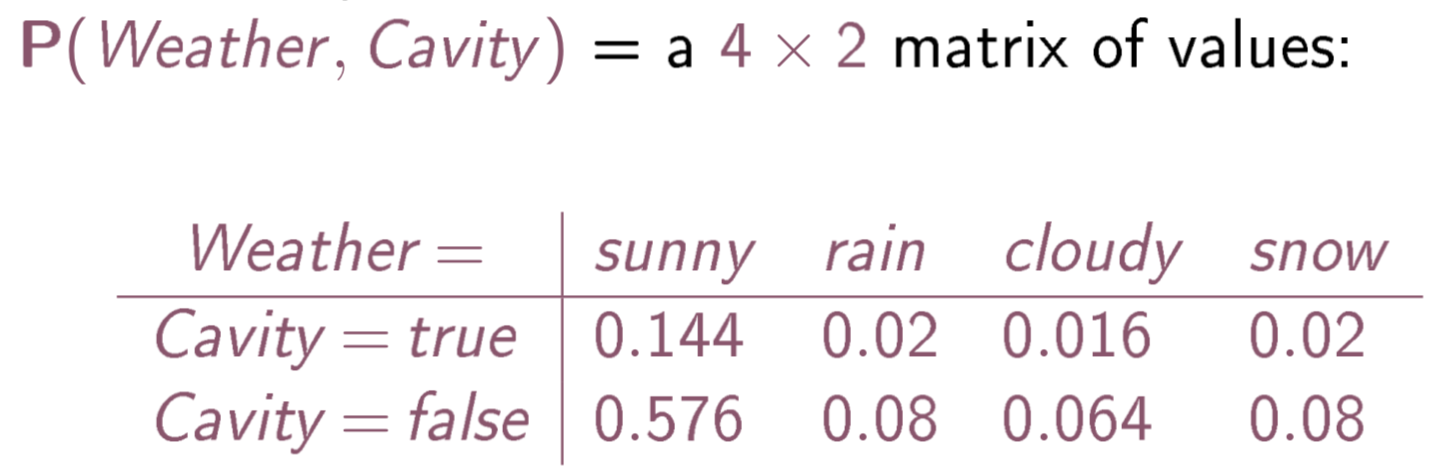
\includegraphics[scale=0.29]{JointProb}
	\end{figure}
\end{multicols}


\subsection*{Probabilità Condizionale}
\addcontentsline{toc}{subsection}{Probabilità Condizionale}
È una probabilità a posteriori, cioè indica come cambia una probabilità dopo una certa evidenza (probabilità di avere una carie sapendo che ho mal di denti; \textbf{P(cavity | Toothache) = 0.6}).\\
Alcune evidenze possono essere irrilevanti: \textbf{P(cavity | Toothache, Sunny) = P(cavity | Toothache)}.
$$ P(A | B) = \frac{P(A \land B)}{P(B)} \text{~~~~~if~} P(B)\neq 0 ~~~~~~~~~~~~~ P(A \land B) = P(A | B) * P(B) = P(B | A) * P(A)$$
\textit{\textbf{Chain Rule}} (si ripete fino ad avere una variabile): $P(X_1, \dots , X_n) = P(X_1, \dots , X_{n-1}) * P(X_n | X_1, \dots , X_{n-1})$
\begin{multicols}{2}
	\noindent
	\textit{\textbf{Normalization}}: con una \textit{costante di normalizzazione} $\alpha$ (Cavity = distribuzione, quando c'è/non c'è la carie).\\
	$P(Cavity|toothache) = \alpha P(Cavity, toothache) = \alpha [P(Cavity, toothache, catch)+P(Cavity, toothache, ¬catch)]$\\
	$= \alpha [\langle 0.108, 0.016\rangle + \langle 0.012, 0.064 \rangle] = \alpha \langle0.12, 0.08 \rangle = \langle 0.6, 0.4\rangle $
	\columnbreak
	\begin{figure}[H]
		\centering
		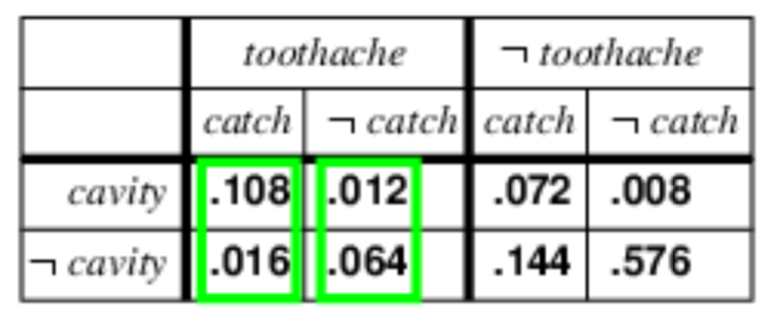
\includegraphics[scale=0.37]{Joint}
	\end{figure}
\end{multicols}
\noindent
\textit{Toothache} è la variabile di evidenza ($E$), \textit{catch} è la variabile nascosta ($H$), \textit{cavity} è la variabile \textit{query} ($Y$).\\
$P(Y|E=e) = \alpha ~P(Y,E=e) = \alpha ~\Sigma_h P(Y,E=e, H=h)$\\
\textit{\textbf{Eventi indipendenti} (per ridurre la tabella)}: $P(A|B) = P(A) ~~or~~ P(B|A) = P(B) ~~or~~ P(A, B) = P(A) * P(B)$
\begin{multicols}{2}
	\noindent
	\textit{\textbf{Bayes' Rule}}: \textit{P(Causa (A)} | \textit{Effetto(B))} $= \frac{P(B | A) * P(A)}{P(B)}$. Dato un effetto, calcola la probabilità di una possibile causa.
	\columnbreak
	\begin{figure}[H]
		\centering
		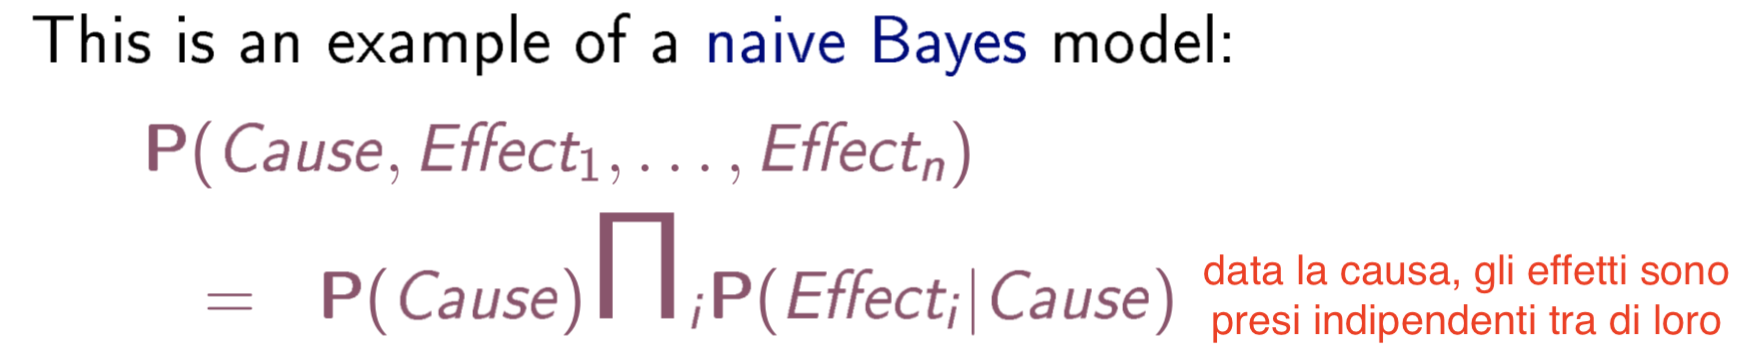
\includegraphics[scale=0.25]{Bayes}
	\end{figure}
\end{multicols}



\chapter*{Decisioni Complesse}
\addcontentsline{toc}{chapter}{Decisioni Complesse}
\begin{multicols}{2}
	\noindent
	Le \textbf{decisioni} corrispondono a \textit{sequenze di azioni}, prese in base al \textit{reward} che si vuole raggiungere. Il valore di un'azione va oltre il beneficio immediato: \textit{utility} a lungo termine (studente a lezione non solo per quella lezione ma per passare l'esame) e acquisire conoscenze. È dunque necessario un framework per prendere decisioni sequenziali e \textit{far fronte all'incertezza}.
	\columnbreak
	\begin{figure}[H]
		\centering
		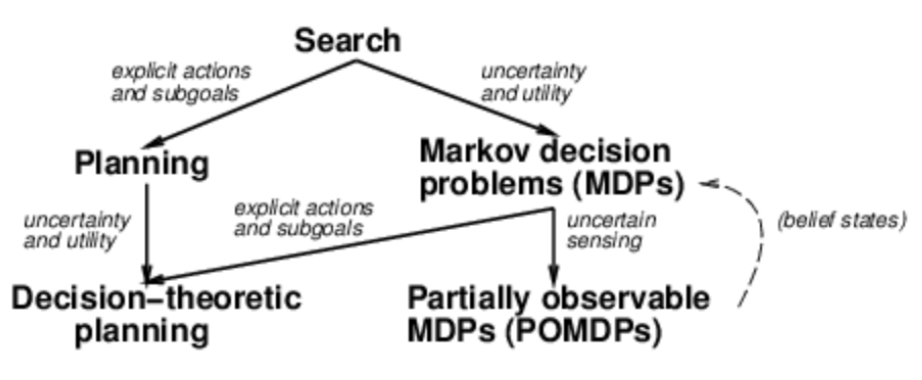
\includegraphics[scale=0.43]{Decision}
	\end{figure}
\end{multicols}
\begin{multicols}{2}
	\noindent
	States $s \in S$, actions $a \in A$\\
	Model $T(s,a,s') \equiv P(s'|s,a) =$ probabilità che $a$ in $s$ vada in $s'$\\
	Reward function $R(s)$ (or $R(s, a)$, $R(s, a, s')$)
	$\begin{cases}
		-0.04 &\text{ (small penalty)  for nonterminal states } \\
		\pm1 & \text{ for terminal states }
	\end{cases}$
	\columnbreak
	\begin{figure}[H]
		\centering
		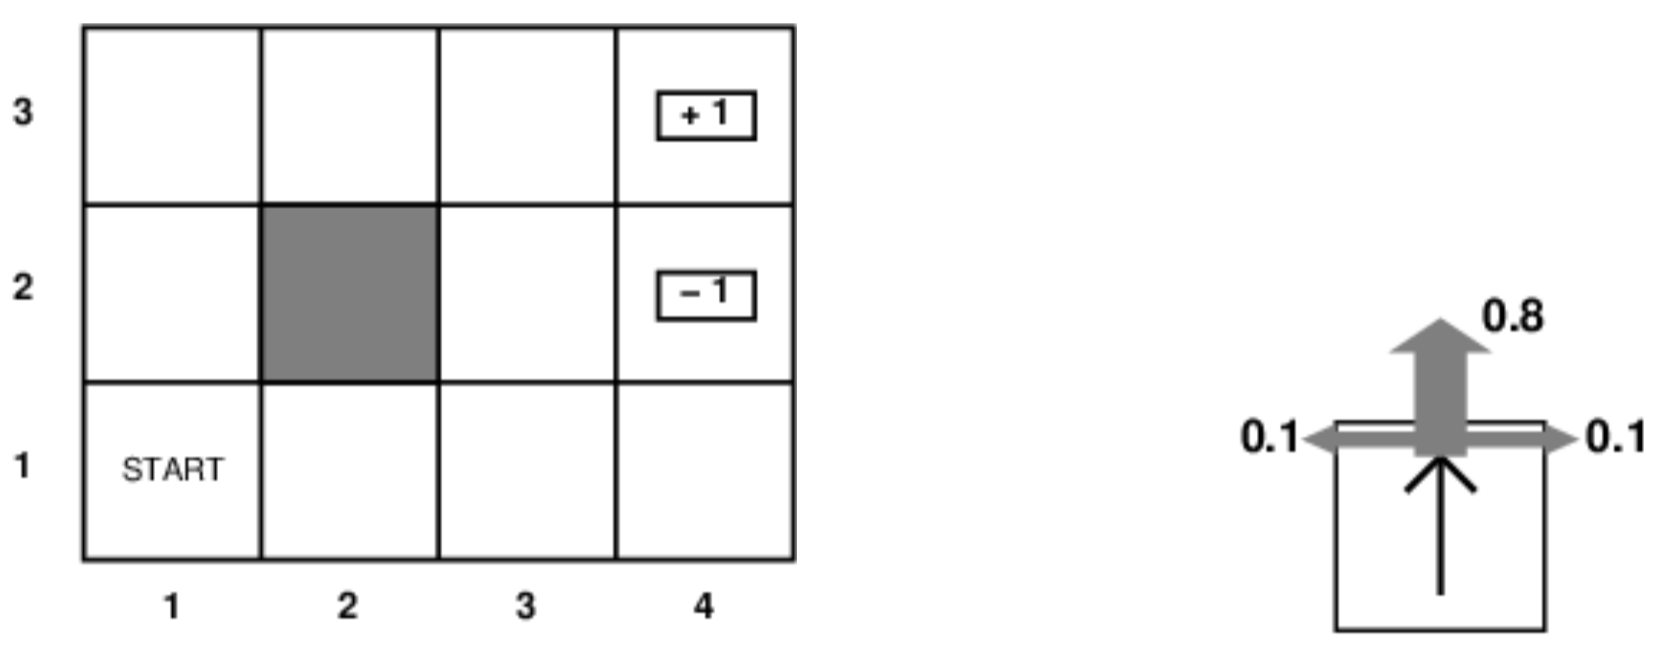
\includegraphics[scale=0.25]{Maze}
	\end{figure}
\end{multicols}
\begin{multicols}{2}
	\noindent
	L'approccio non è ottimo perché è sconveniente valutare tutte le sequenze senza considerare il risultato reale ($\mathcal{O}(k^t n^t)$ con $k$ azioni, $t$ stages e $n$ risultati). È complesso stimare l'\textit{utility} di una sequenza rispetto a quella di un singolo stato.\\
	Per trovare una sequenza ottimale si usa una \textit{\textbf{policy} ottimale} $\pi(s)$ che massimizza la somma attesa dei rewards.
	\columnbreak
	\begin{figure}[H]
		\centering
		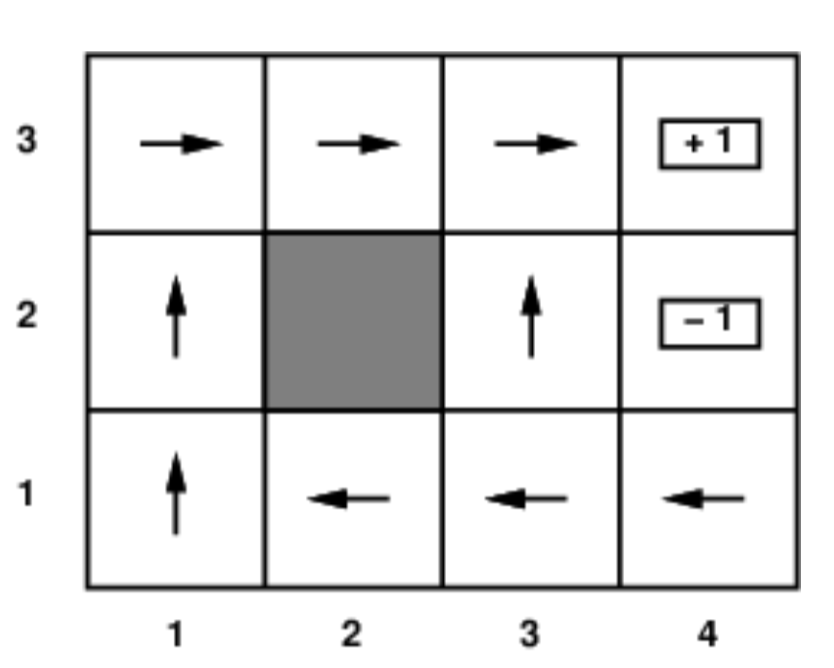
\includegraphics[scale=0.25]{Maze2}
	\end{figure}
\end{multicols}


\section*{Decision Trees}
\addcontentsline{toc}{section}{Decision Trees}
\begin{multicols}{2}
	\noindent
	L'idea principale è un approccio backward dalle foglie, facendo uso della \textit{Maximum Expected Utility (MEU)}.\\\\
	Il valore di un nodo foglia $C$ è: $EU(C)$.\\\\
	Il valore di un \textit{Chance Node C} (cerchi) è:\\$EU(C) = \Sigma_{D\in Child(C)} PR(D)EU(D)$\\\\
	Il valore di un \textit{Decision Node D} (quadrati) è:\\$EU(D) = max_{C\in Child(D)} EU(C)$\\\\
	La \textit{policy} massimizza l'utility di un decision node:\\
	$\pi(D) = arg max_{C\in Child(D)} EU(C)$
	\columnbreak
	\begin{figure}[H]
		\centering
		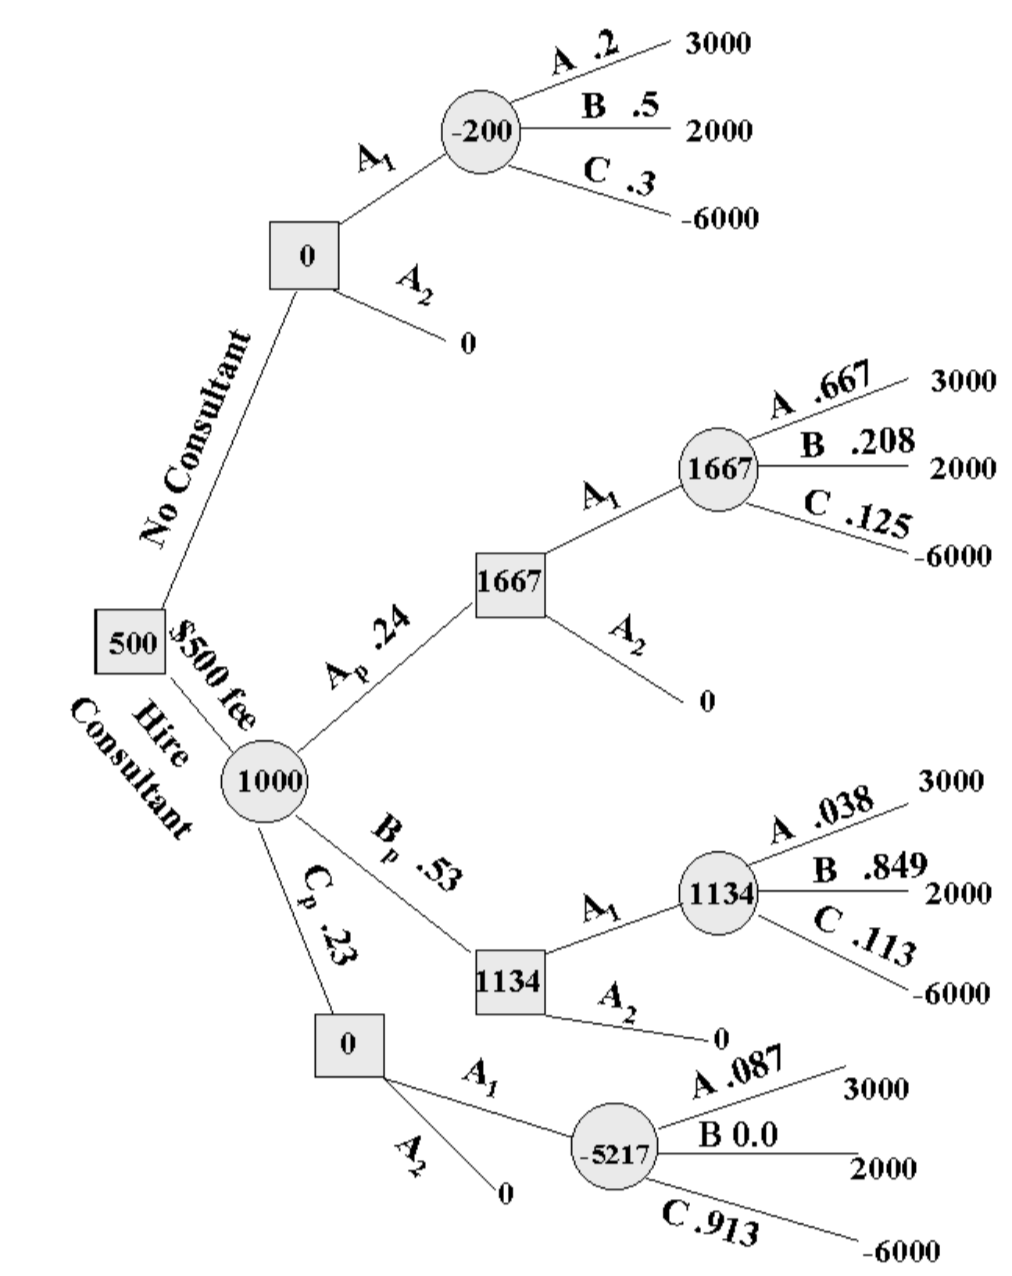
\includegraphics[scale=0.27]{DecTree}
	\end{figure}
\end{multicols}


\section*{Markov Decision Processes}
\addcontentsline{toc}{section}{Markov Decision Processes}
I \textit{\textbf{Markov Decision Problems}} sono una classe generica di problemi di ricerca non-deterministici (più generali e meno strutturati dei \textit{decision trees}; possono avere cicli).\\
Ci sono quattro componenti $(S, A, R, Pr)$:
\begin{itemize}
	\item $S$ è un insieme finito di stati ($|S| = n$);
	\item $A$ è un insieme finito di azioni ($|A| = m$);
	\item una \textit{funzione di transizione} $Pr$: $p(s', a, s) = Pr\{ S_{t+1} = s' | S_t = s, A_t = a \}$;
	\item \textit{real valued reward function} $R$: $r(s', a, s) = \mathbb{E}[R_{t+1} | S_{t+1} = s', A_t = a, S_t, s]$. ($\mathbb{E}$ = \textit{expected value}).
\end{itemize}
Nei \textit{Markov Decision Problems} le azioni/stati passati sono irrilevanti quando si prendono decisioni (solo stato corrente).\\
Non dipende dalla storia e dal tempo (stazionarietà). È \textit{completamente osservabile}: non si predice esattamente lo stato futuro ma conosciamo quello presente.
$$Pr\{R_{t+1}, S_{t+1} | S_t, A_t\} = Pr\{R_{t'+1}, S_{t'+1} | S_t', A_t'\} ~~~\forall t, t'$$

\noindent
Ci sono principalmente tre tipi di \textit{policies}:
\begin{itemize}
	\item \textit{Non stazionaria}: $\pi: S \times T \rightarrow A$. $\pi (s, t)$ azione allo stato $s$ con $t$ stati al termine;
	\item \textit{Stazionaria}: $\pi: S \rightarrow A$. $\pi (s)$ azione per lo stato $s$ (senza guardare il tempo);
	\item \textit{Stocastica}: $\pi(a | s)$ probabilità di scegliere l'azione $a$ nello stato $s$ (non la vedremo).
\end{itemize}


\subsection*{Policy non stazionaria}
\addcontentsline{toc}{subsection}{Policy non stazionaria}
\textit{Value function}: $V: S \rightarrow \mathfrak{R}$. Associa un valore considerando i rewards accumulati nel tempo.\\
$v_\pi(s)$ denota il valore della policy $\pi$ per lo stato $s$.\\
Il problema si ha quando ci sono infinite sequenze di stati (e di conseguenza un numero infinito di reward). Soluzioni:
\begin{itemize}
	\item Si sceglie un limite finito (\textit{horizon}) che può essere un numero fissato di passi;
	\item \textit{stato assorbente}: garantisce che per ogni policy verrà raggiunto uno stato terminale;
	\item uso del \textit{discounting} $\gamma$: uso una funzione per dare più importanza ai reward nuovi rispetto a quelli vecchi.\\
	Più $\gamma$ è piccolo e più si ragiona sul presente. I reward recenti hanno un'\textit{utility} più alta di quelli vecchi.
	\newline
\end{itemize}

\noindent
\textit{\textbf{Value}} di uno stato $s$ seguendo la policy $\pi$: si accumulano i reward (\textit{discounted});~~~ $v_\pi(s) = \mathbb{E}\{\Sigma_{k=0}^\infty \gamma^k r_{t+k+1} | s_t = s \}$

\noindent
\textit{\textbf{Q-Value} (action value or quality function)} prendendo l'azione $a$ nello stato $s$ seguendo la policy $\pi$;
$$q_\pi(s, a) = \Sigma_{s'} p(s' | a, s) (r(s, a, s')+\gamma v_\pi(s')) ~~~~~ \text{dove }~ v_\pi(s) = q_\pi(s, \pi(s))$$

\subsubsection*{Bellman Equations}
\addcontentsline{toc}{subsubsection}{Bellman Equations}
Il valore dello stato iniziale deve essere uguale al valore \textit{discounted} dello stato successivo atteso, più il reward atteso lungo il percorso: ~~~$v_\pi(s)=\Sigma_{s'} p(s'|\pi(s),s)(r(s,\pi(s),s')+\gamma v_\pi(s'))$\\\\
\textit{\textbf{Optimal policy}}: $\pi_*(s)$ è una policy ottimale sse $v_{\pi_*}(s) \geq v_\pi(s) ~~\forall s, \pi$.\\
\textit{\textbf{Optimal value}}:$v_*(s) = max_\pi v_\pi (s)$ expected utility partendo da $s$ e agendo da lì in poi in modo ottimale.\\
\textit{\textbf{Optimal action-value function}}: $q_*(a, s) = max_\pi q_\pi(s, a)$.\\\\
$v_*(s)$ è il valore ottimo, dunque la \textit{consistency condition} può essere scritta come segue:
$$v_*(s) = max_{a\in \mathcal{A}(s)} q_*(s, a) = max_{a\in \mathcal{A}(s)} \Sigma_{s'} p(s' | a, s) (r(s, a, s') + \gamma v_*(s')) $$
\noindent
In altre parole: prima l'azione era data dalla \textit{policy}, ora l'azione è quella migliore.

\newpage
\subsubsection*{Value Iteration}
\addcontentsline{toc}{subsubsection}{Value Iteration}
\begin{multicols}{2}
	\noindent
	Si trasforma l'equazione di Bellman combinando \textit{policy evaluation} (calcolando $v_\pi$ di una data policy) e la \textit{policy improvement} (cioè l'aggiornamento dei valori, rendendo $\pi$ greedy rispetto a $v_\pi$). Il metodo risultante \textbf{Value Iteration} è una successiva approssimazione.\\
	Salva il valore di ogni stato per produrre la nuova stima della value function ($k+1$ stage).
	\columnbreak
	\begin{figure}[H]
		\centering
		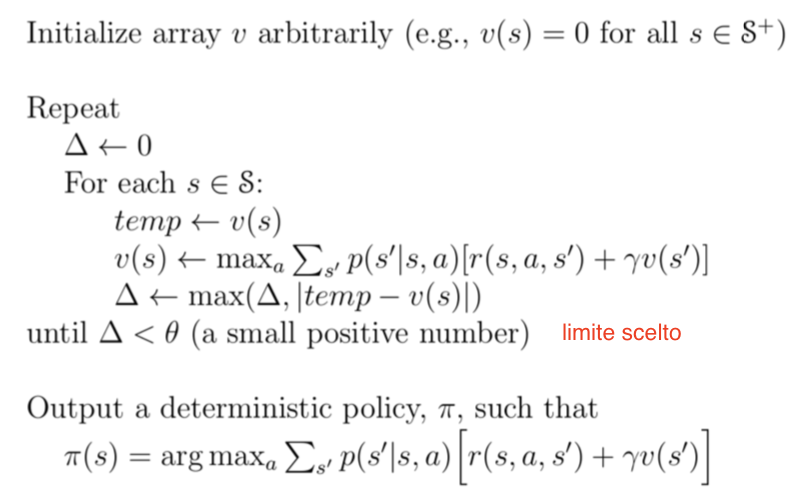
\includegraphics[scale=0.33]{VI}
	\end{figure}
\end{multicols}
\noindent
\textit{\textbf{Bellman backup}}: ~$v^{k+1}(s) = max_a \Sigma_{s'} P(s' | a, s) (r(a, s, s') + \gamma v^k(s'))$
\begin{multicols}{2}
		\begin{figure}[H]
		\centering
		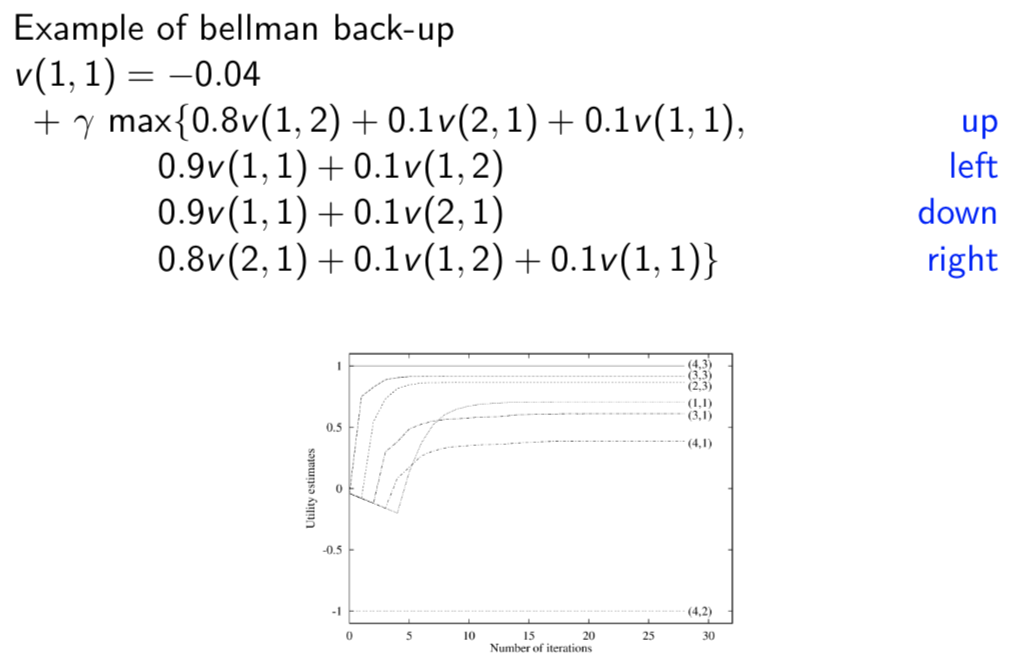
\includegraphics[scale=0.30]{VI1}
	\end{figure}
	\columnbreak
	\begin{figure}[H]
		\centering
		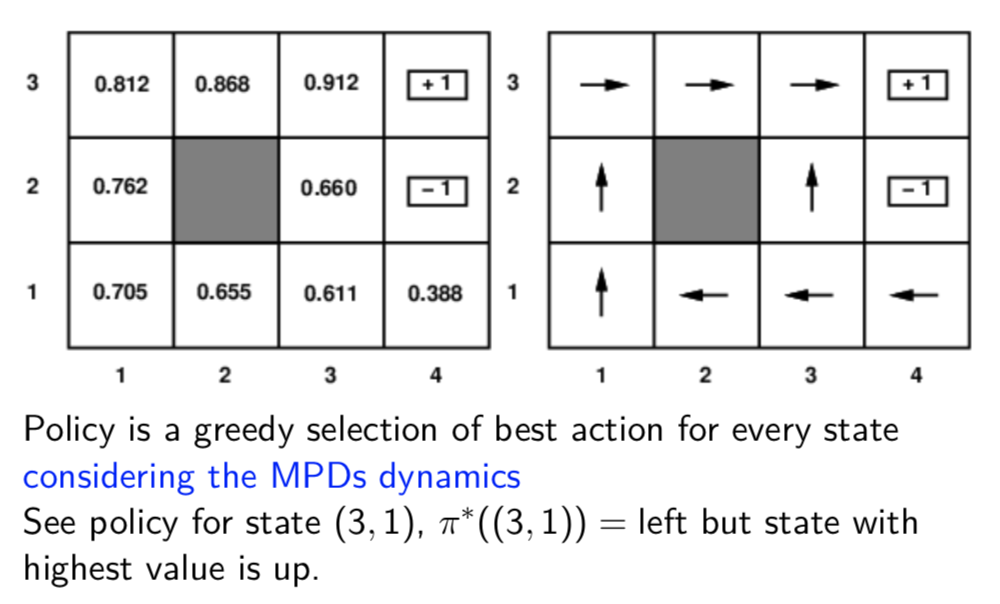
\includegraphics[scale=0.32]{VI2}
	\end{figure}
\end{multicols}
\noindent
\textit{Value Iteration} garantisce la convergenza ad una funzione di valore ottimale. \textit{Complessità} quadratica nel numero numero di stati e lineare nel numero di azioni.


\subsubsection*{Policy Iteration}
\addcontentsline{toc}{subsubsection}{Policy Iteration}
Si sceglie una policy iniziale arbitraria poi ri ripete il seguente passaggio fino a quando $\pi$ non viene modificata: dato $\pi$ calcolare le utilities (\textit{policy evaluation}) e aggiornare $\pi$ con le nuove utilities (\textit{policy improvement}).\\
\begin{multicols}{2}
	\noindent
	Per calcolare le utilities data una policy $\pi$ (\textbf{policy evaluation}): ~~$v(s) = \Sigma_{s'} p(s' | s, \pi(s)) (r(s, \pi(s), s') + \gamma v(s'))$\\
	Si risolvono $n$ equazioni lineari in $n$ incognite (complessità $\mathcal{O}(n^3)$).\\\\
	\textbf{Policy improvement}: dati i valori di ogni stato $v(s)$, se il valore di uno stato può essere migliorato, si adotta la nuova azione nella policy.\\\\
	L'algoritmo itera fino a quando non ci sono più miglioramenti. La policy trovata sarà sicuramente ottimale.
	\columnbreak
	\begin{figure}[H]
		\centering
		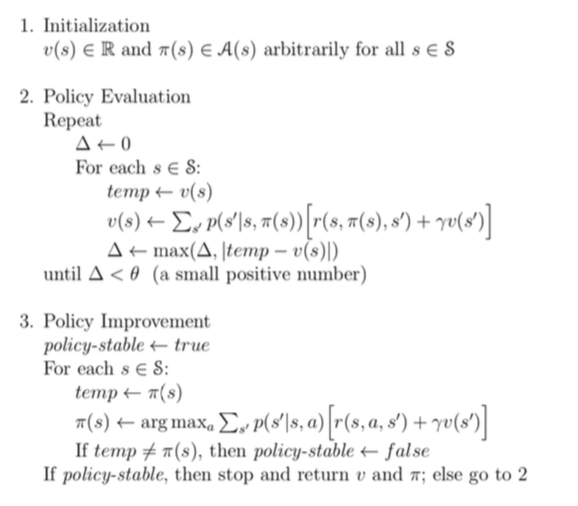
\includegraphics[scale=0.49]{PI}
	\end{figure}
\end{multicols}
\noindent
La policy iteration converge spesso in poche iterazione ma è molto dispendioso. È necessario modificarla.\\\\
\textit{\textbf{Modified Policy Iteration}}: si fanno alcuni passi di \textit{value iteration} (ma con $\pi$ fissato) partendo dalla value function prodotta l'ultima volta, per produrre un passo di valutazione con policy approssimata.\\
Converge molto più velocemente di \textit{Value Iteration} e \textit{Policy Iteration}.



\chapter*{Bayesian Network}
\addcontentsline{toc}{chapter}{Bayesian Network}
Una notazione grafica per le asserzioni di indipendenza condizionale e dunque per la specifica compatta della \textit{full joint distribution}; sintassi:
\begin{multicols}{2}
	\begin{itemize}
		\item un insieme di nodi, uno per variabile;
		\item un grafo diretto aciclico (il collegamento indica "influenza direttamente");
		\item una distribuzione condizionale per ogni nodo, dati i suoi padri ~~$P(X_i | Parents(X_i))$
	\end{itemize}
	\noindent
	Nel caso più semplice, una distribuzione condizionale è rappresentata come una \textit{Conditional Probability Table (CPT)}, dando una distribuzione su $X_i$ per ogni combinazione di valori del padre.
	\columnbreak
	\begin{figure}[H]
		\centering
		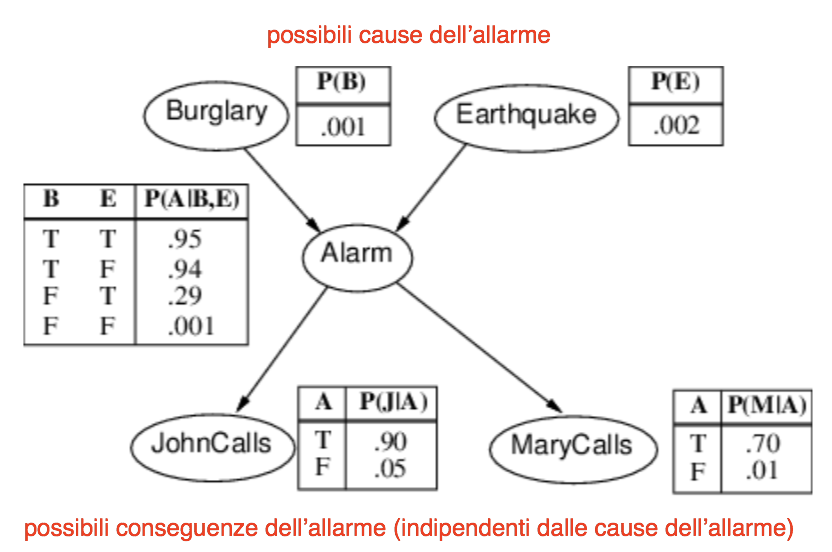
\includegraphics[scale=0.42]{BN}
	\end{figure}
\end{multicols}

\noindent
Usando questa network e dividendo dunque le tabelle dei vari nodi, abbiamo una CPT per ogni nodo $X_i$ con $2^k$ righe ($k$ = parents($X_i$). Se ogni nodo non ha più di $k$ padri, la rete completa richiede $\mathcal{O}(n * 2^k)$, invece di $\mathcal{O}(2^n)$.
\begin{multicols}{2}
	\noindent
	\textit{\textbf{Global Semantics}}: definisce la \textit{full joint distribution} come il prodotto delle distribuzioni locali condizionali.
	\begin{figure}[H]
		\centering
		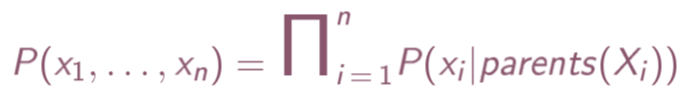
\includegraphics[scale=0.42]{BN1}
	\end{figure}
	\columnbreak
	\begin{figure}[H]
		\centering
		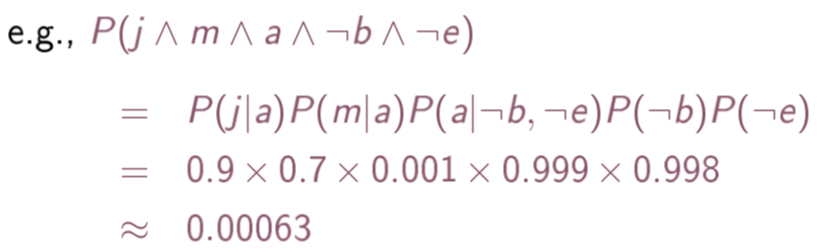
\includegraphics[scale=0.42]{BN2}
	\end{figure}
\end{multicols}

\noindent
\textit{\textbf{Local Semantics}}: ogni nodo è condizionalmente indipendente dai suoi non-discententi, dati i suoi padri.\\
\textit{\textbf{Teorema}}: \textit{Local Semantics} $\iff$ \textit{Global Semantics}\\\\
\textit{\textbf{Markov Blanket}}: ogni nodo è condizionalmente dipendente dai nodi presenti nella sua markov blanket.
\begin{center}
\textit{\textbf{Markov blanket} = parents + children + children's parents}
\end{center}


\section*{Costruzione di una Bayesian Network}
\addcontentsline{toc}{section}{Costruzione di una Bayesian Network}
È necessario un metodo tale che una serie di asserzioni localmente verificabili di indipendenza condizionale garantisca la semantica globale richiesta.
\begin{multicols}{2}
	\begin{itemize}
		\item si scegli un ordine di variabili $X_1, \dots, X_n$;
		\item per $i$ da $1$ a $n$, si aggiunge $X_i$ alla rete e si selezionano i padri tali che\\
		$P(X_i | Parents(X_i)) = P(X_i | X_1, \dots, X_{i-1})$
	\end{itemize}
	La scelta dei padri garantisce la semantica globale.
	\columnbreak
	\begin{figure}[H]
		\centering
		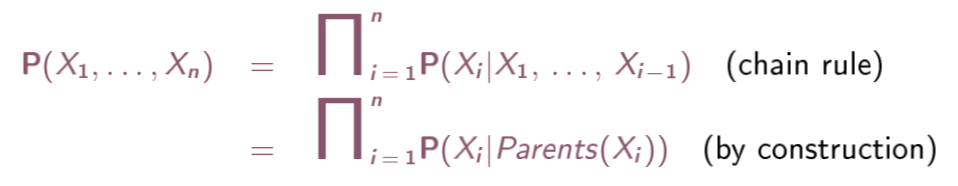
\includegraphics[scale=0.42]{BN3}
	\end{figure}
\end{multicols}
\begin{multicols}{2}
	\begin{figure}[H]
		\centering
		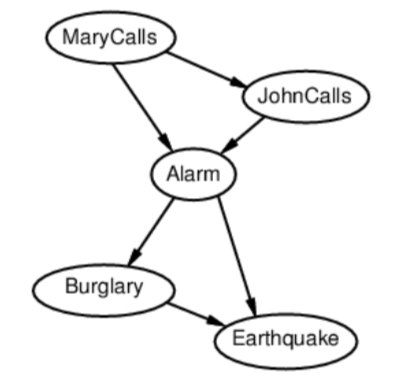
\includegraphics[scale=0.29]{BN4}
	\end{figure}
	\columnbreak
	\begin{figure}[H]
		\centering
		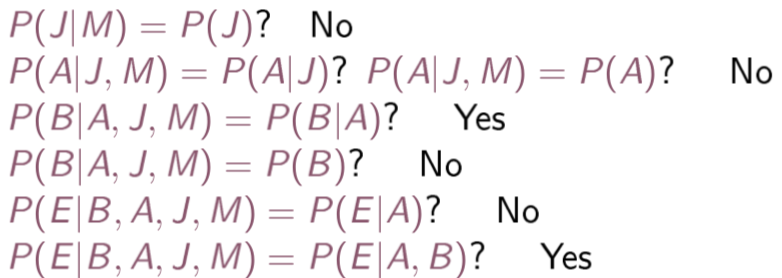
\includegraphics[scale=0.37]{BN5}
	\end{figure}
\end{multicols}
\noindent
Nell'esempio abbiamo scelto prima gli effetti e poi le cause, rendendo complessa la decisione per le indipendenze condizionali. Il grafico inoltre diventa meno compatto e più confuso (aumentando le righe delle rispettive tabelle).


\section*{Compact Conditional Distributions}
\addcontentsline{toc}{section}{Compact Conditional Distributions}
\begin{multicols}{2}
	\noindent
	Le \textit{CPT} crescono esponenzialmente nel numero dei padri. La soluzione sono delle \textit{distribuzioni canoniche compatte}, che rendono lineare il n° di parametri nel n° di padri.\\
	\textit{\textbf{Noisy-Or distributions}}: è una rappresentazione delle cause indipendenti tra loro. Vengono considerate solo alcune cause, dunque si può aggiungere un \textit{leak node} per raggruppare tutte le altre possibili.
	\columnbreak
	\begin{figure}[H]
		\centering
		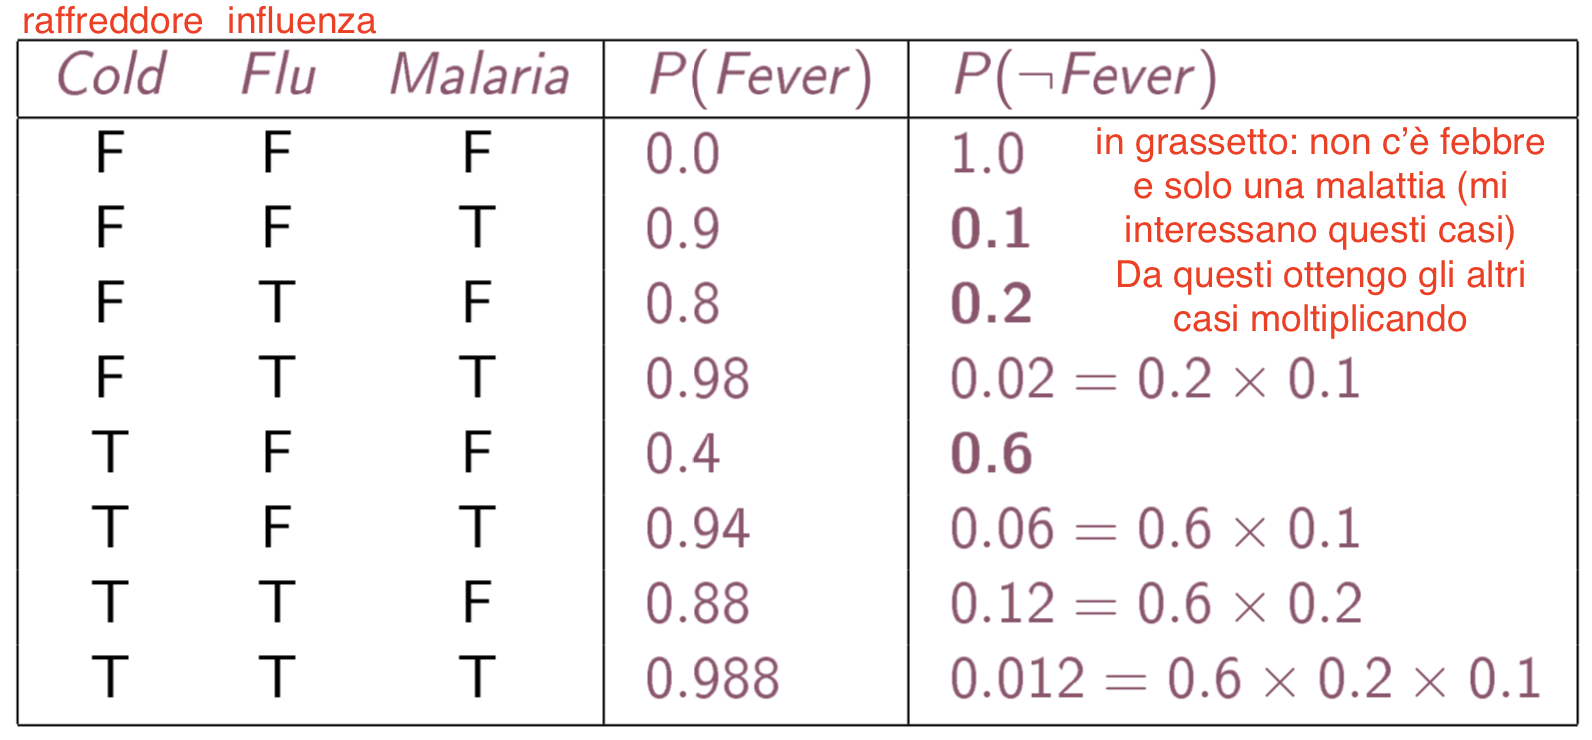
\includegraphics[scale=0.21]{Tab}
	\end{figure}
\end{multicols}
\noindent
\textit{\textbf{Simple Query}}: calcola a posteriori probabilità marginali (togliendo le variabili che non interessano) ~$P(X_i | E=e)$\\
Ci sono due algoritmi per le simple query: \textit{Enumeration Algorithm} e \textit{Variable Elimination}.\\\\
\textit{\textbf{Inference by Enumeration}}: un metodo utile per sommare delle variabili del joint senza darne la rappresentazione esplicita. Riscrive la \textit{full joint} usando il prodotto delle righe della CPT. I nodi dipenderanno solo dai padri.
$$P(B|j, m) = \alpha P(B) ~\Sigma_e P(e) ~\Sigma_a P(a | B, e) P(j | a) P(m | a) $$

\subsection*{Enumeration Algorithm}
\addcontentsline{toc}{subsection}{Enumeration Algorithm}
\begin{multicols}{2}
\begin{figure}[H]
	\centering
	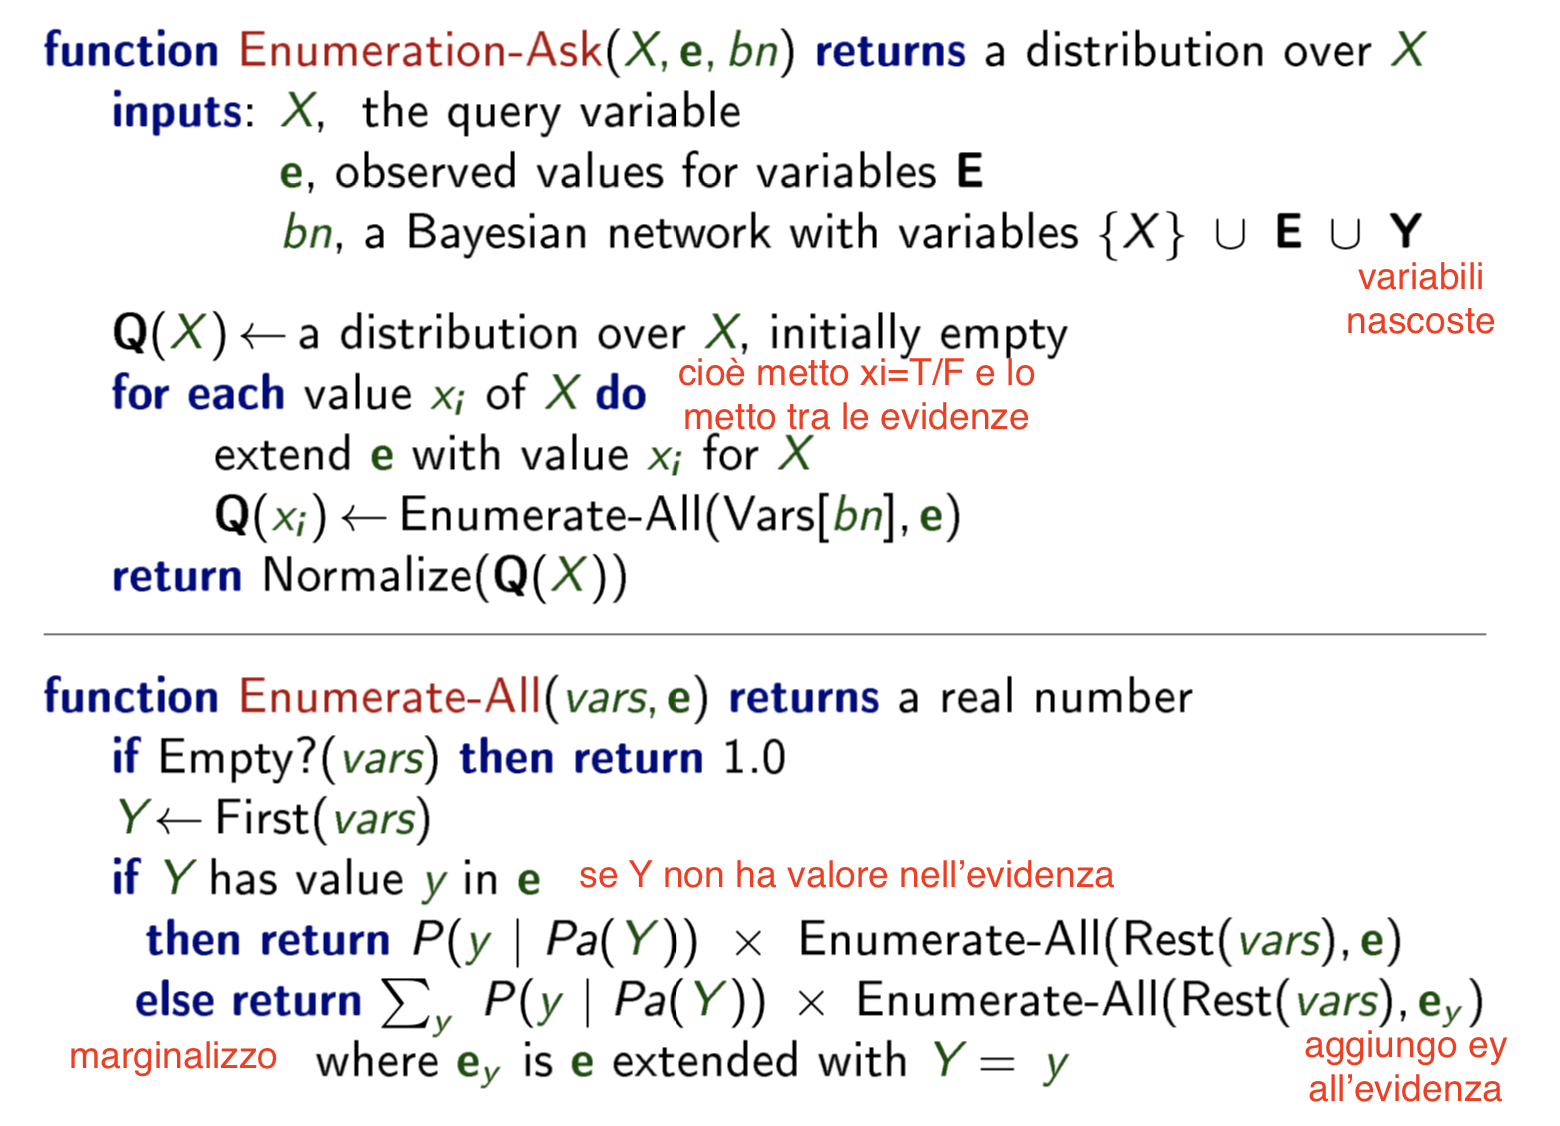
\includegraphics[scale=0.25]{Alg}
\end{figure}
	\columnbreak
	\begin{figure}[H]
		\centering
		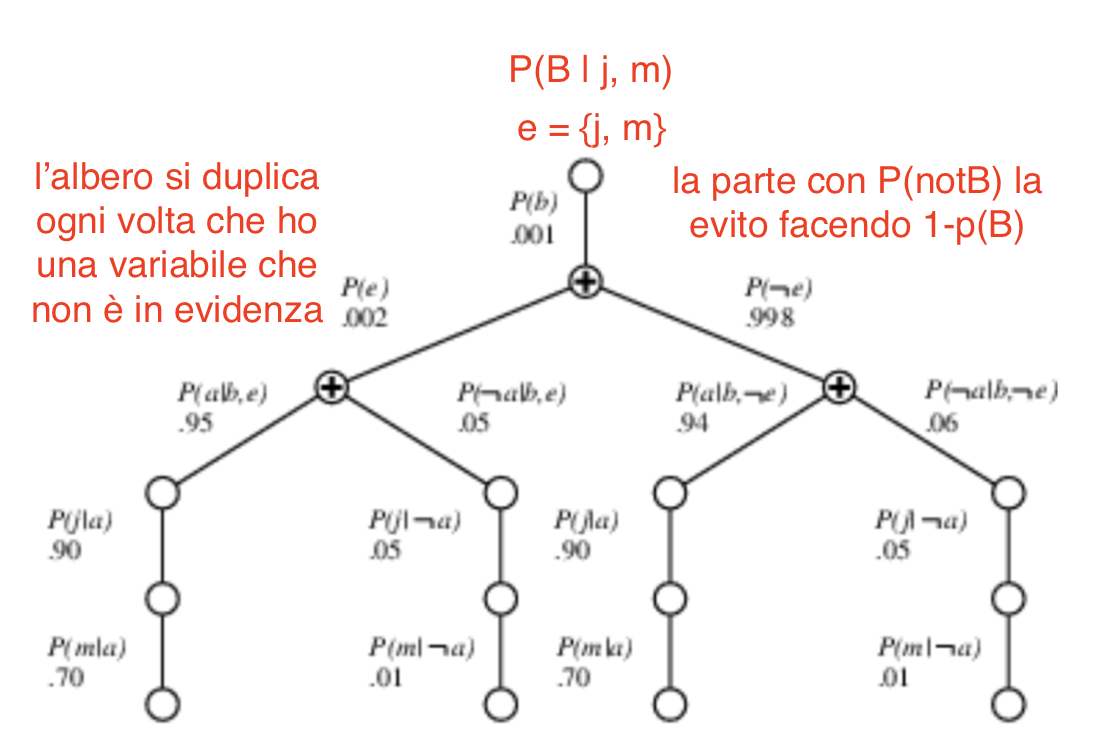
\includegraphics[scale=0.30]{Alb}
		\caption*{L'enumerazione è inefficiente perchè ho calcoli ripetuti.}
	\end{figure}
\end{multicols}


\subsection*{Variable Elimination}
\addcontentsline{toc}{subsection}{Variable Elimination}
Risolve le sommatorie da destra a sinistra, tenendo i risultati parziali (\textit{fattori}) per evitare calcoli ripetuti.
\begin{multicols}{2}
	\begin{figure}[H]
		\centering
		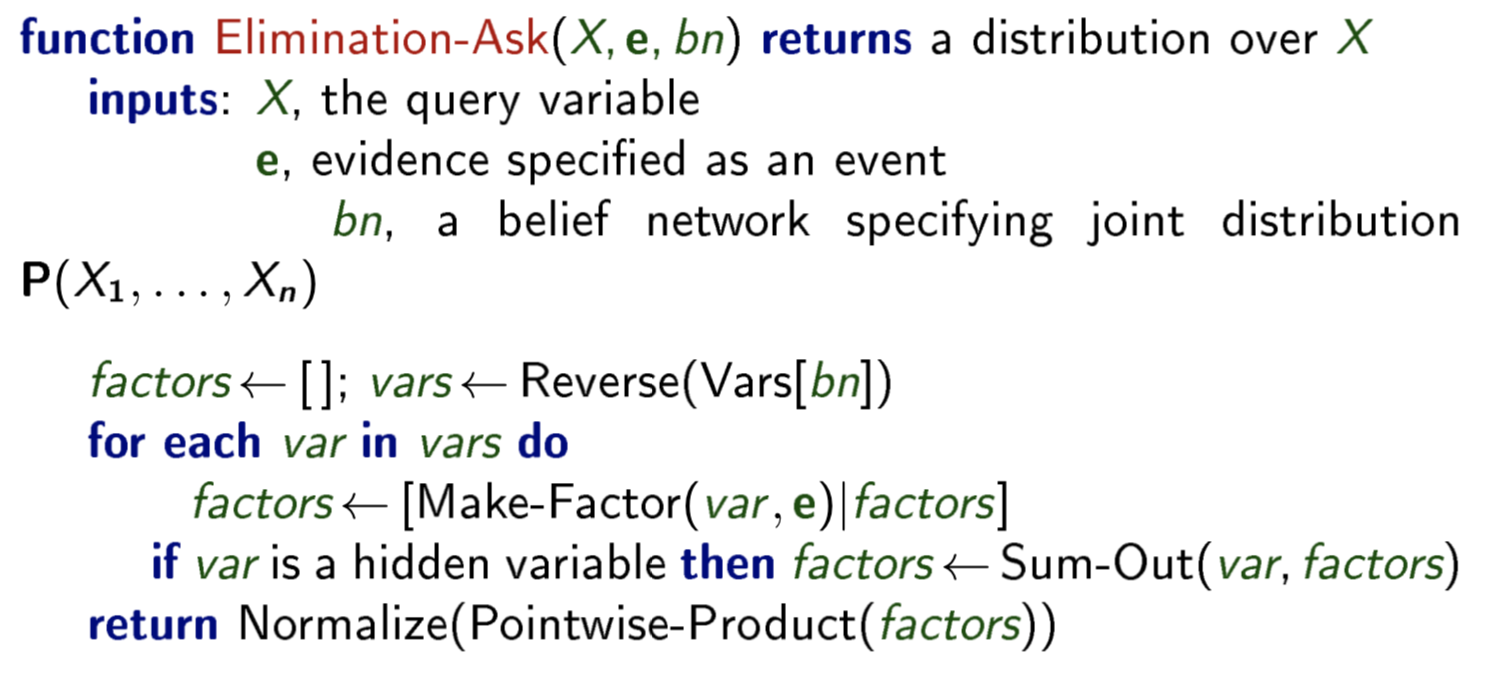
\includegraphics[scale=0.26]{Alg2}
	\end{figure}
	\columnbreak
	\begin{figure}[H]
		\centering
		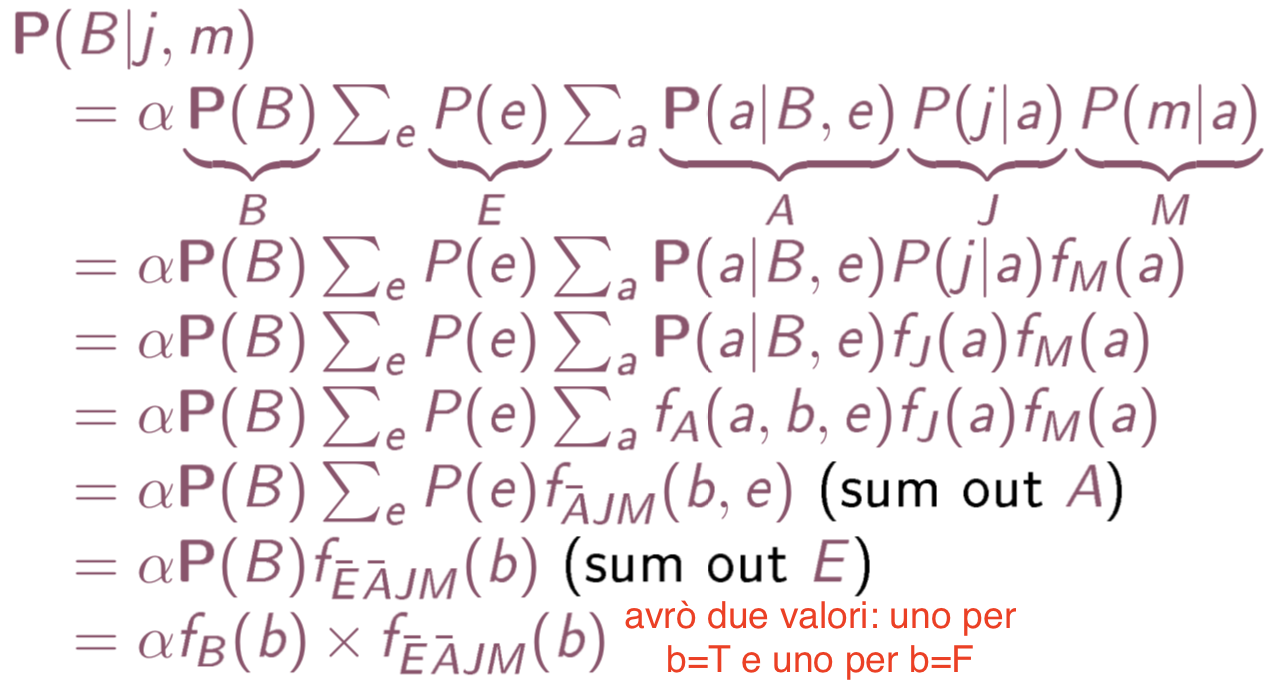
\includegraphics[scale=0.25]{VarEl}
	\end{figure}
\end{multicols}

\subsection*{Irrelevant Variables}
\addcontentsline{toc}{subsection}{Irrelevant Variables}
Data $P(B|j, m) = \alpha P(B) ~\Sigma_e P(e) ~\Sigma_a P(a | B, e) P(j | a) P(m | a) $, la variabile $m$ è irrilevante (somma $= 1$).\\
\textit{\textbf{Teorema 1}}: $Y$ è irrilevante a meno che $Y\in$ \textit{Anchestors}$(\{X\} \cup E)$.\\
\textit{\textbf{Moral Graph} di una Bayes Net}: si collegano i padri e si tolgono le frecce (non è più un grafo diretto).\\
$A$ è \textbf{\textit{m-separato}} da $B$ a causa di $C$, sse sono separati da $C$ nel \textit{moral graph}.\\
\textit{\textbf{Teorema 2}}: $Y$ è irrilevante se è $E$ lo m-separa da $X$. ~$P(J | A=true)$, $B$ ed $E$ sono irrilevanti.

\subsection*{Approximate Inference by Stocastic Simulation}
\addcontentsline{toc}{subsection}{Approximate Inference by Stocastic Simulation}
\textit{\textbf{Prior Sampling}}: si prende un ordine topologico e si fanno i vari \textit{sample} (sequenze) tenendo conto della probabilità. Per ogni sequenza si calcola la probabilità stimata $\hat{P}(F, F, F, T, F) = \frac{X}{N}$, con $X =$ n° di occorrenze del \textit{sample}.\\
\textit{\textbf{Rejection Sampling}}: rigetto i \textit{sample} che non sono in accordo con l'evidenza. Per ogni \textit{sample} valido computo $N[J=F] = +1$ oppure $N[J=T] = +1$, aggiungendo ad $\langle 0, 0 \rangle$. Infine si normalizza trovando il $P(J | b)$ cercato.



\chapter*{Reinforcement Learning}
\addcontentsline{toc}{chapter}{Reinforcement Learning}
\textit{Idea di base}: imparare a mappare le situazioni alle azioni, per massimizzare la sequenza di reward.\\
Si fanno tentativi/test ed errori mentre si interagisce con l'ambiente. Interesse per i reward a lungo termine.\\
Una MDP  che non conosce le dinamiche non sa quali sono gli stati buoni e dove portano le azioni.\\
Ci sono due approcci, uno fa uso di modelli, l'altro di campioni:
\begin{itemize}
	\item \textit{\textbf{Model-Based}}: cerca di imparare un modello evitando stati/azioni non buoni, riducendo i passi di esecuzione e facendo un uso efficiente di dati.
	\item \textit{\textbf{Model-Free}}: impara \textit{Q-function} e \textit{policy} direttamente; è più semplice perché non ha bisogno di un modello.
	\newline
\end{itemize}

\textit{\textbf{Esempio}}: si vuole calcolare la media attesa dell'età di una classe (~$\mathbb{E} [A] = \Sigma_a P(a) ~a$~), con i due approcci.
\begin{itemize}
	\item \textit{\textbf{Model-Based}}: si stima $\hat{P}(a) = \frac{num(a)}{N}$, dove $num(a)$ è il n° di studenti con età $a$. Abbiamo $\mathbb{E} [A] \approx \Sigma_a P(a) * a$
	\item \textit{\textbf{Model-Free}}: non c'è stima. Abbiamo ~$\mathbb{E} [A] \approx \frac{1}{N} \Sigma_i a_i$~~ dove $a_i$ è l'età della persona $i$ presa da un campione.
\end{itemize}


\section*{Model-Based}
\addcontentsline{toc}{section}{Model-Based}
Si stima $P(x)$ dai sample acquisiti $x_i \sim P(x)$. Si stima $\hat{P}(x) = count(x)/k$.
Si stima $\hat{T}(s, a, s')$ dai sample acquisiti ($s_0, a_0, s_1, a_1, s_2 \dots$). Si stima il modello $\hat{T}(s, a, s') = \frac{count(s_{t+1}=s', a_t=a, s_t=s)}{count(s_t=s, a_t = a)}$.
\begin{multicols}{2}
	\begin{figure}[H]
		\centering
		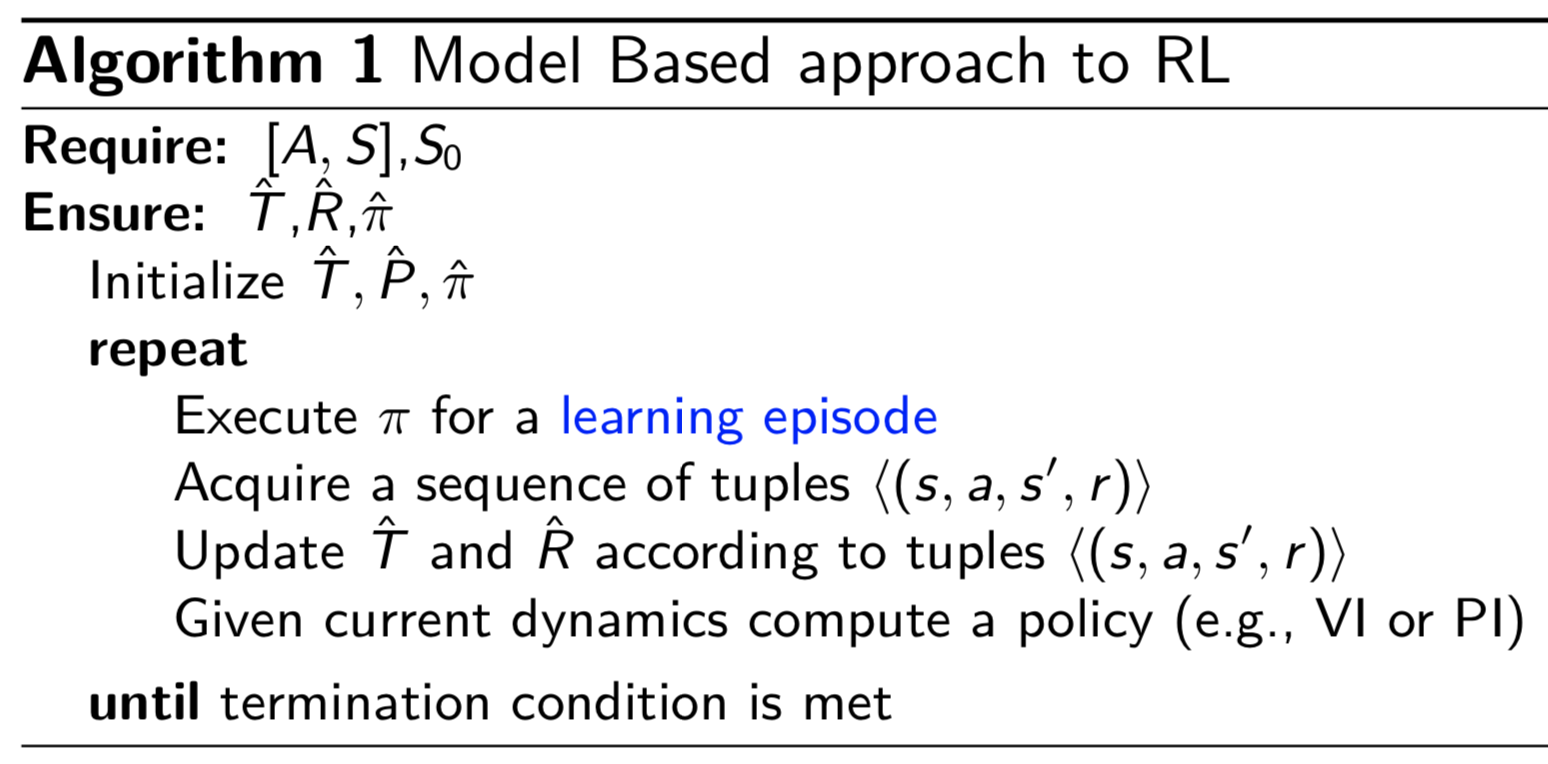
\includegraphics[scale=0.23]{RL}
	\end{figure}
\columnbreak
	\noindent
	La durata del \textit{learning episode} è data da quando uno stato terminale viene raggiunto oppure vengono fatti un certo numero di time-step.\\\\
	Esegue sempre l'azione migliore, dato il modello corrente; non c'è esplorazione.
\end{multicols}


\section*{Model-Free}
\addcontentsline{toc}{section}{Model-Free}
Si vuole calcolare un'aspettativa pesata di $P(x)$: ~$\mathbb{E}[f(x)] = \Sigma_x P(x) ~f(x)$.\\
Questo approccio stima l'aspettativa direttamente dai sample: $x_i \sim P(x), \mathbb{E}[f(x)] \approx \frac{1}{N} \Sigma_i f(x_i)$.\\\\
Si valuta la \textit{Value Function} dall'esperienza.: si esegue $\pi$ per alcuni \textit{learning episodes}, si calcola il \textit{discounted} reward ogni volta che si visita uno stato e infine si calcola la media sui sample.\\\\
\textit{\textbf{Sample-Based Policy Evaluation}}:data la formula di Bellman $V_\pi^{k+1}(s) = \Sigma_{s'} T(s, \pi(s), s') (R(s, \pi(s), s') + \gamma V_\pi^k(s'))$\\
Questa viene applicata ad $N$ sample (rimuovendo $T$): ~$sample_i = R(s, \pi(s), s_i') + \gamma V_\pi^k(s_i')$\\
Si fa calcola poi la media su tutti i sample: ~$V_\pi^{k+1}(s) = \frac{1}{N} ~\Sigma_i ~sample_i$\\
\\
\textit{\textbf{Temporal Difference Learning}}: si impara da ogni esperienze, non dopo un episodio. Si aggiorna $V(s)$ dopo ogni azione, dato $(s, a, s', r)$ ottenuto.\\
\textit{Update} $V_\pi(s)$: ~~$V_\pi(s) \leftarrow (1 - \alpha) V_\pi(s) + \alpha(R(s, \pi(s), s') + \gamma V_\pi(s')))$ ~ decrementando $\alpha$ ad ogni passo.

\subsection*{Q-Learning}
\addcontentsline{toc}{subsection}{Q-Learning}
Si vuole calcolare la policy basata su $V(s)$ senza usare direttamente $V$.\\
\textit{Q-Learning}: sample based Q-Value iteration.\\
$Q_{k+1}(s, a) = \Sigma_{s'} ~T(s, a, s')(R(s, a, s') + \gamma max_{a'} ~Q_k(s', a'))$\\\\
\textit{\textbf{Proprietà di Q-Learning}}: converge alla policy ottima se si esplora abbastanza e se si rende il \textit{learning rate} piccolo abbastanza (ma non decresce così velocemente).\\
\textit{Off Policy Learning}: imparare la policy ottimale senza seguirla (la scelta delle azioni non impatta sulla convergenza).
\begin{multicols}{2}
	\begin{figure}[H]
		\centering
		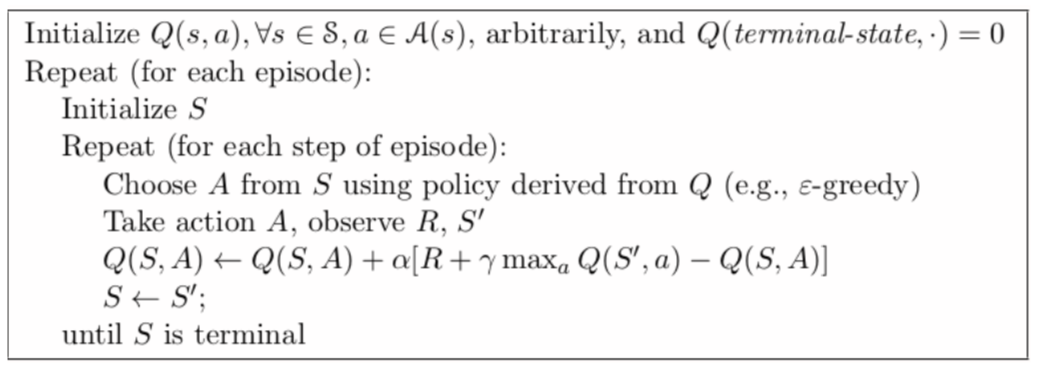
\includegraphics[scale=0.32]{QL}
	\end{figure}
	\columnbreak
	\noindent
	$\epsilon$\textit{-greedy}: sceglie la miglior azione la maggior parte delle volte, ma alcune volte (con probabilità $\epsilon$) scegli un'azione in modo randomico tra tutte le azioni (con uguale probabilità).
\end{multicols}

\subsection*{SARSA}
\addcontentsline{toc}{subsection}{SARSA}
\begin{multicols}{2}
	\begin{figure}[H]
		\centering
		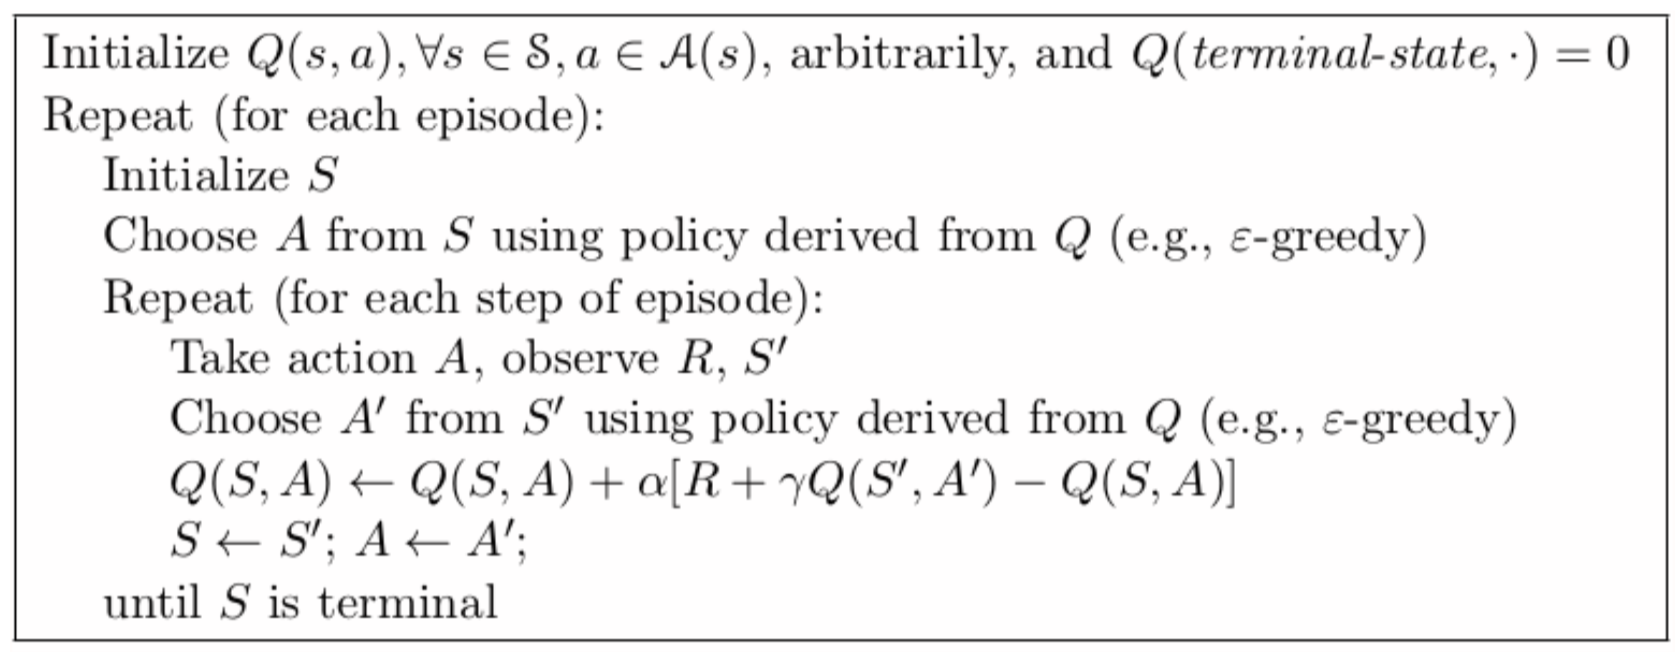
\includegraphics[scale=0.20]{SARSA}
	\end{figure}
	\columnbreak
	\noindent
	\textit{\textbf{SARSA}}: deriva dalla tupla $(S, A, R, S', A')$\\\\
	È caratterizzata dal fatto che si calcola l'azione successiva basandosi sulla policy (on-policy).	
\end{multicols}
\begin{multicols}{2}
	\noindent
	\textit{Q-Learning} impara la policy ottimale ma occasionalmente fallisce a causa della selezione dell'azione $\epsilon$\textit{-greedy}.\\\\
	\textit{SARSA}, essendo on-policy, ha una migliore on-line performance.
	\columnbreak
	\begin{figure}[H]
		\centering
		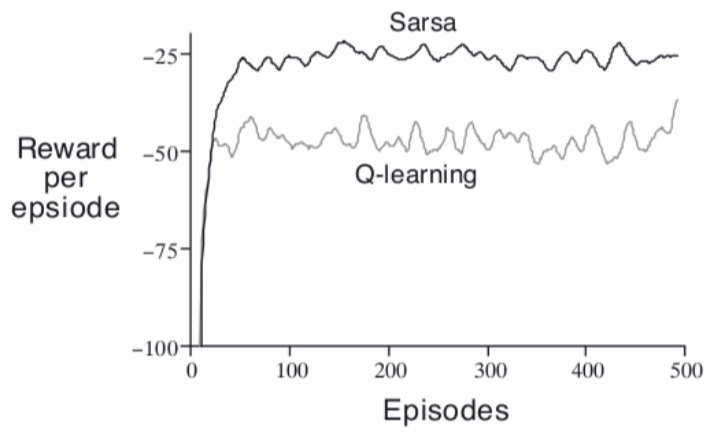
\includegraphics[scale=0.27]{QvsS}
	\end{figure}	
\end{multicols}

\noindent
\textit{\textbf{The Exploration vs Exploiting Dilemma}}
\begin{itemize}
	\item \textit{Exploration}: serve per migliorare la value function e massimizzare il reward; però esplorare parti irrilevanti causa una perdita di tempo.
	\item \textit{Exploiting}: usare la conoscenza per non perdere tempo esplorando parti irrilevanti.
\end{itemize}
Ci sono due metodi principali:
\begin{itemize}
	\item $\epsilon$\textit{-greedy}: scegliere in modo greedy la maggior parte delle volte (probabilità $1-\epsilon$) e in maniera randomica con probabilità $\epsilon$.
	\item \textit{Soft-max (or Boltzmann)}:
\end{itemize}





\end{document}